\subsection{Numerical Results and Their Implications}\label{sec:p2p:results}

%\begin{figure*}[bt]
%\begin{minipage}[b]{0.32\textwidth}
%	\centering
%	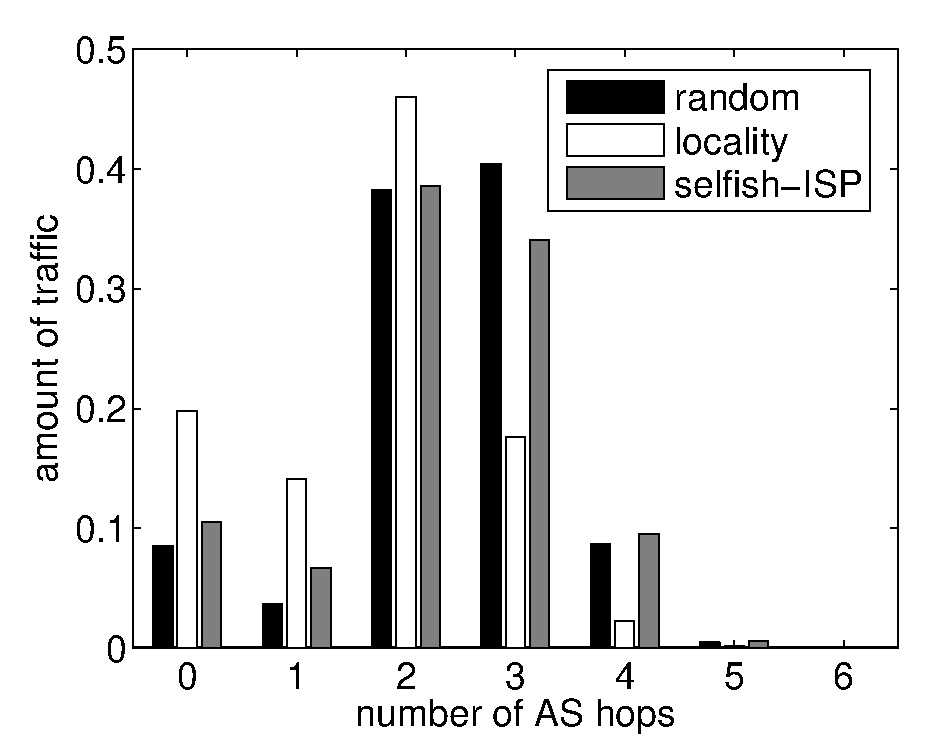
\includegraphics[width=0.95\textwidth]{aslevel/p2p/results/figs/hops}
% 	\caption{Distribution of AS path lengths weighted by the amount of traffic.}
% 	\label{fig:CDF_hops}
%\end{minipage}
%\hspace{0.01\textwidth}
%\begin{minipage}[b]{0.32\textwidth}
%	\centering
%	\includegraphics[width=\textwidth]{aslevel/p2p/results/figs/outgoing}
% 	\caption{Total outgoing AS traffic for different peer selection strategies.}
% 	\label{fig:outgoing}
%\end{minipage}
%\hspace{0.01\textwidth}
%\begin{minipage}[b]{0.32\textwidth}
%	\centering
%	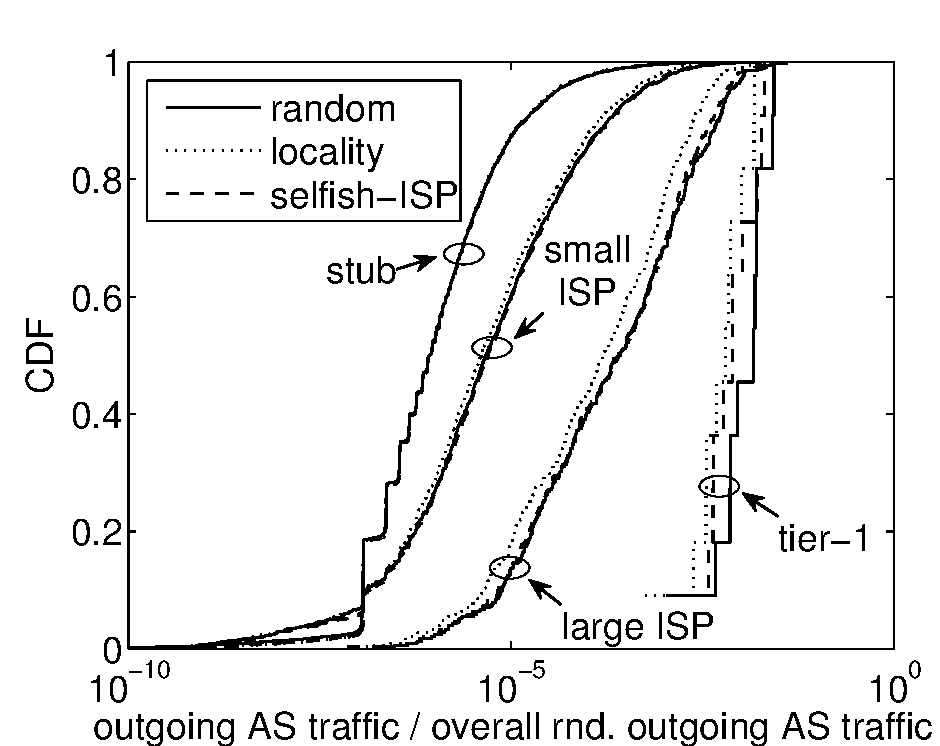
\includegraphics[width=\textwidth]{aslevel/p2p/results/figs/outgoing_CDF}
% 	\caption{CDF of the outgoing AS traffic grouped by AS size.}
% 	\label{fig:outgoing_CDF}
%\end{minipage}
%\end{figure*}

% \begin{figure*}[bt]
% \begin{minipage}[t]{0.49\textwidth}
% 	\centering
% 	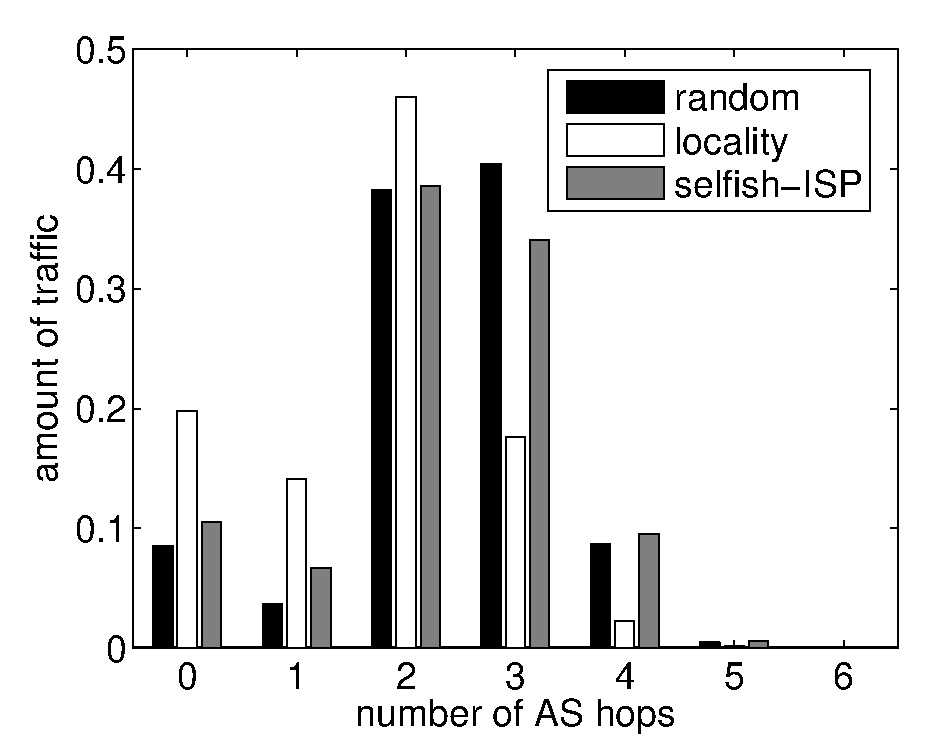
\includegraphics[width=\textwidth]{aslevel/p2p/results/figs/hops}
%  	\caption{Distribution of AS path lengths weighted by the amount of traffic.}
%  	\label{fig:CDF_hops}
% \end{minipage}
% \hspace{0.01\textwidth}
% \begin{minipage}[t]{0.49\textwidth}
% 	\centering
% 	\includegraphics[width=\textwidth]{aslevel/p2p/results/figs/outgoing}
%  	\caption{Total outgoing AS traffic for different peer selection strategies.}
%  	\label{fig:outgoing}
% \end{minipage}
% \end{figure*}

\begin{figure}[bt]
\centering
	\includegraphics[width=0.5\textwidth]{aslevel/p2p/methodology/figs/npeers_perTier}
 	\caption{Ratio of peers per ISP class aggregated over all swarms in the measurement set.}
 	\label{fig:npeers_perTier}
\end{figure}

\begin{figure}[bt]
\centering
	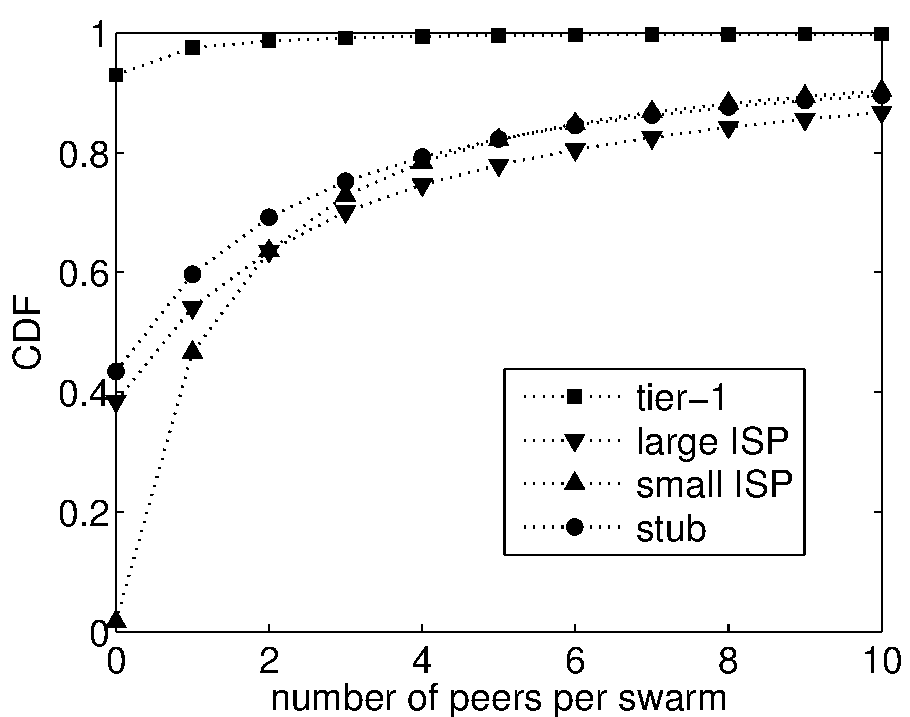
\includegraphics[width=0.7\textwidth]{aslevel/p2p/methodology/figs/CDF_npeers_perswarm}
	\caption{CDF of the number of peers per swarm depending on the different ISP classes.}
	\label{fig:CDF_npeers_perswarm}
\end{figure}

\begin{figure}[bt]
\centering
	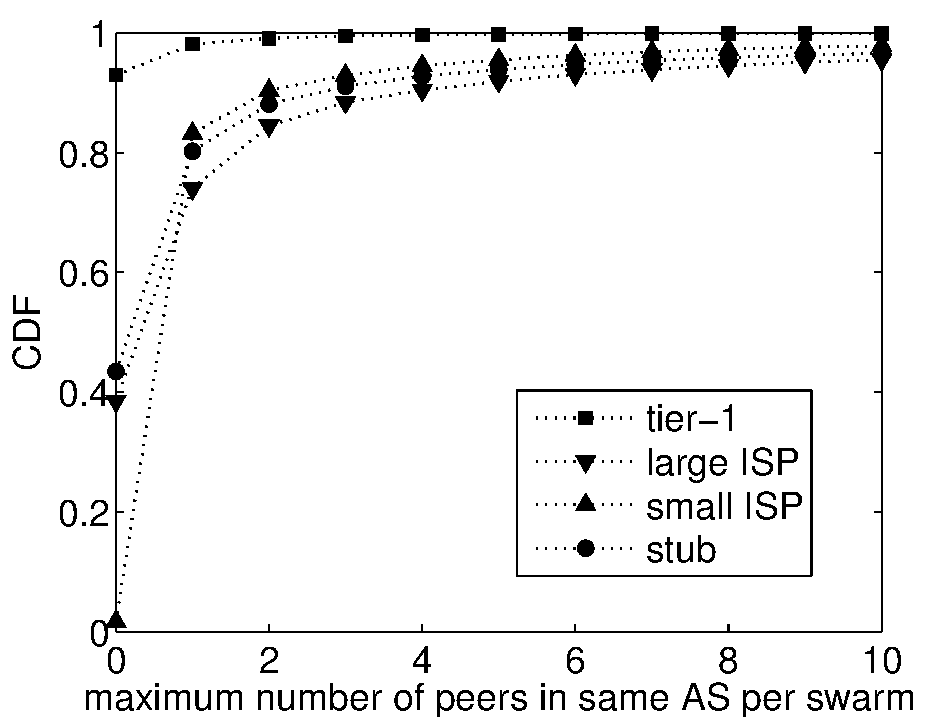
\includegraphics[width=0.7\textwidth]{aslevel/p2p/methodology/figs/CDF_maxpeers_perswarm_perAS}
	\caption{CDF of the maximum number of peers in same AS per swarm depending on the tier.}
	\label{fig:CDF_maxpeers_perswarm_perAS}
\end{figure}

In this section we present the numerical results obtained by applying our methodology to the measurement data and describe their importance for ISPs. First we show how the peers are distributed over the different ASs. Then we characterize the traffic emerged by BitTorrent swarms and investigate the impact of locality and selfish-ISP peer selection algorithm. Finally, we estimate the transit costs arising by the BitTorrent swarms and investigate the potential of ISPs to maximize their balance by the peer selection algorithms.

\subsubsection{Distribution of Peers in the Internet Hierarchy}

In the following we describe how peers of BitTorrent swarms are distributed over the Internet.
Figure~\ref{fig:npeers_perTier} shows the distribution of peers over the different tiers. The peers of all torrents are considered. Most of the peers are in large ISP ASs, where \unit[40]{\%} of all peers are located. In small ISP and stub ASs a similar amount of \unit[29]{\%} and \unit[31]{\%} of the peers is located, respectively. Only very few peers are located in \tier ASs, which is less than \unit[1]{\%} of all peers in all swarms. Hence, the access to peers by \tier ASs is negligible. That means that \tier ASs barely have an impact on ALTO mechanisms that control only the peers of the own AS.

Figure~\ref{fig:CDF_npeers_perswarm} shows the cumulative distribution function (CDF) of peers per swarm. We summed up the number of peers being in the same tier for each swarm and calculated the CDF. The probability that at least one peer in a small ISP is existing in a swarm is highest. Only about \unit[2]{\%} of the swarms do not contain any small ISP peer. About \unit[57]{\%} of the swarms contain stub AS peers and more than \unit[60]{\%} contain peers from large ISPs. The probability to find more than one peer of non \tier ASs is about \unit[45]{\%} for small ISPs and a bit higher for large ISPs and stub ASs. There are less than \unit[10]{\%} of the swarms which contain a peer from \tier. Finding more than one peer of \tier ASs in one swarm is very unlikely. Few swarms have a very large number of peers, with the maximum of 9467 peers of one distributed over all large ISPs.

% \begin{figure}[bt]
% 	\centering
% 	\includegraphics[width=\figwidth\textwidth]{figs/npeers_perTier.eps}
%  	\caption{Number of peers in each tier. All swarms are considered.}
%  	\label{fig:npeers_perTier}
% \end{figure}

% \begin{figure}[bt]
% 	\centering
% 	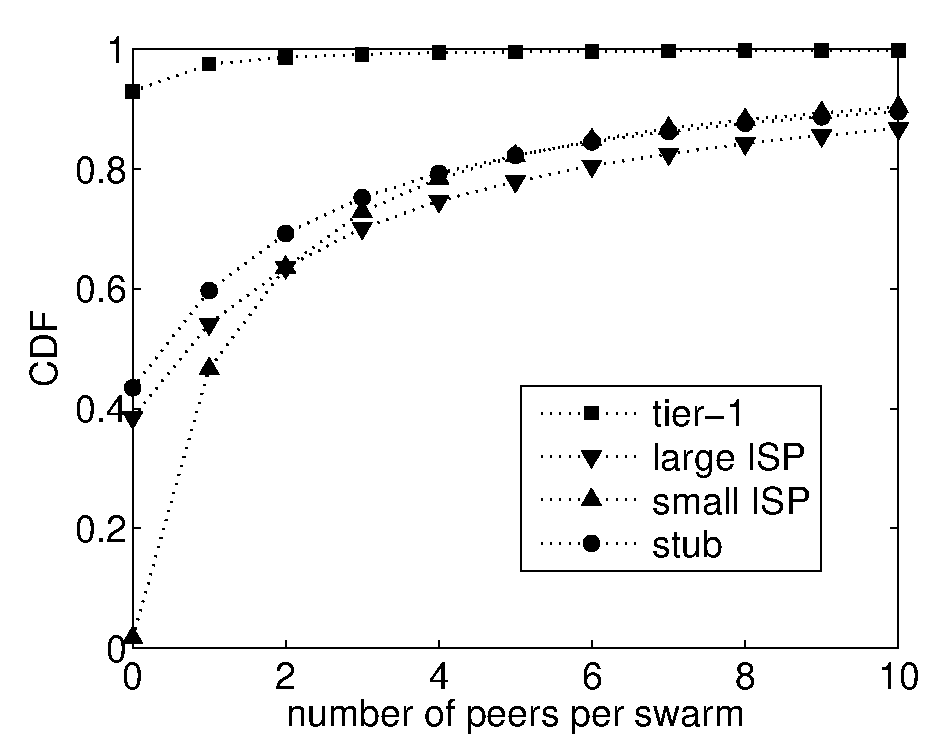
\includegraphics[width=\figwidth\textwidth]{figs/CDF_npeers_perswarm.eps}
%  	\caption{Cumulative probability of the number of peers per swarm for each tier.}
%  	\label{fig:CDF_npeers_perswarm}
% \end{figure}

% \begin{figure}[bt]
% 	\centering
% 	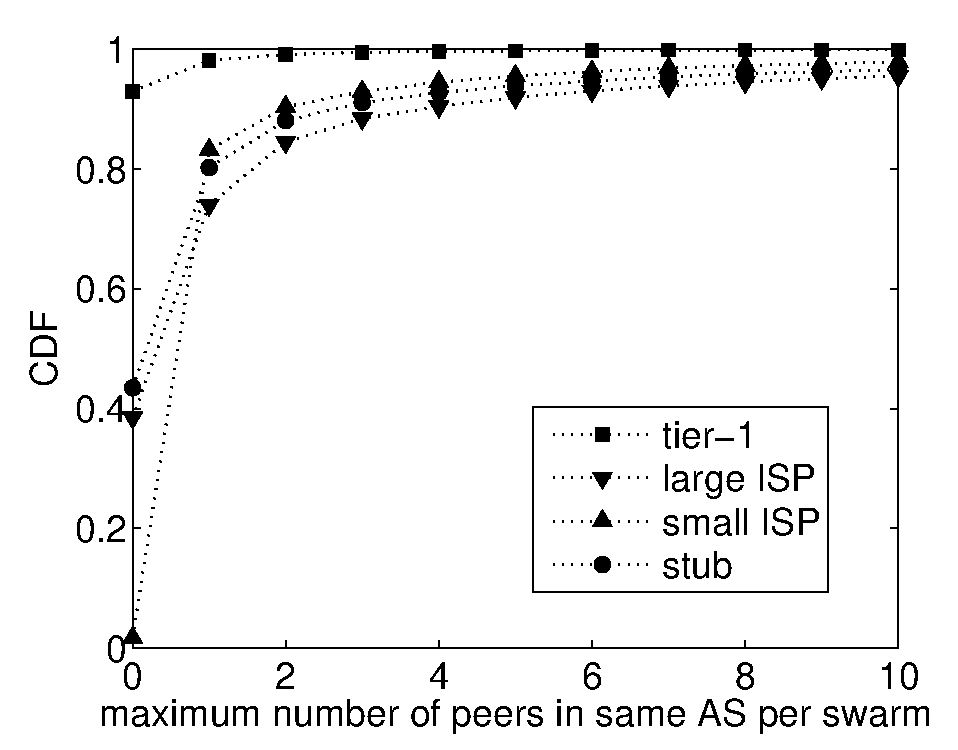
\includegraphics[width=\figwidth\textwidth]{figs/CDF_maxpeers_perswarm_perAS.eps}
%  	\caption{Cumulative probability of the maximum number of peers in same AS per swarm.}
%  	\label{fig:CDF_maxpeers_perswarm_perAS}
% \end{figure}

Peers can exchange data locally in the same AS as soon as at least two of them are in it. This cannot be derived from \reffig{fig:CDF_npeers_perswarm}, since peers can be located in the same tier, but not in the same AS.
In \reffig{fig:CDF_maxpeers_perswarm_perAS} we calculated the cumulative probability of the maximum number of peers in a swarm which are located in the same AS. As soon as the maximum number of peers in one AS is at least 2, data can be exchanged by the peers locally. Figure~\ref{fig:CDF_maxpeers_perswarm_perAS} shows that the probability to exchange traffic locally is low and that large ISPs have the greatest potential. In about \unit[15]{\%} of the large ISPs, peers find neighbors being located in the same AS. For small ISP and stub ASs the chance to find peers of the same swarm in the same AS is about \unit[10]{\%} and \unit[12]{\%} respectively. Hence, considering all ASs the potential for local neighbor selection is relatively small, intra-AS traffic is only generated in \unit[15]{\%} and less of non \tier ASs. But there are a few swarms with many peers generating a lot of traffic which have a very high potential for traffic optimization. The AS with the most peers in one swarm is a large ISP containing 3372 peers of one swarm. The dataset contains 42 swarms with more than 1000 peers in a single AS.
%Inline with \cite{Hossfeld2011}?.
In \tier ASs there is barely no chance to connect to a local neighbor.

\subsubsection{Traffic Characteristics for P2P Guidance Strategies}
In this subsection we characterize the traffic produced by BitTorrent swarms. Further on we investigate the potential of ALTO techniques to optimize the swarm in terms of load on the network and AS path length.
First we look at the traffic characteristics of the standard BitTorrent algorithm and in the following we compare the different selection strategies.
The number of AS hops is the number of ASs on the AS path connecting two peers without regarding the source AS. The number of hops are weighted by $L(\alpha,\beta)$, i.e. the amount of traffic and the number of concurring AS paths, see \refequ{equ:linkload}. Figure~\ref{fig:CDF_hops} shows the amount of traffic on AS paths with length in AS hops for the different selection strategies. The median is about 2 AS hops if peers are selected randomly. Most traffic is on paths with two or three AS hops without selection strategy. Paths are up to 10 AS hops in the investigated swarms.

\begin{figure}[bt]
	\centering
	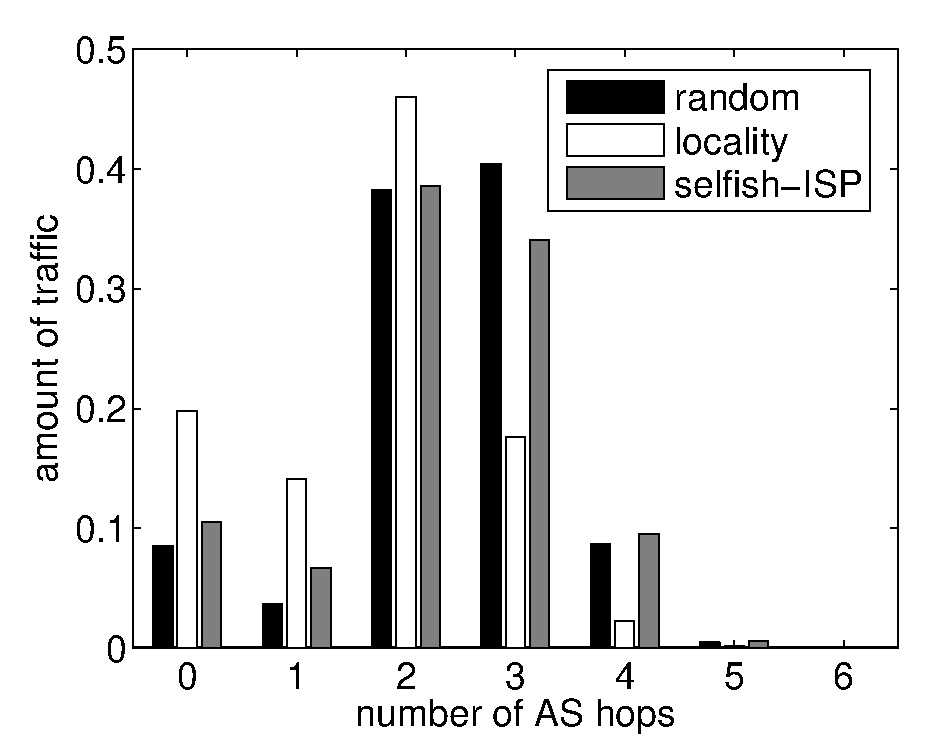
\includegraphics[width=0.7\textwidth]{aslevel/p2p/results/figs/hops}
 	\caption{Distribution of AS path lengths weighted by the amount of traffic.}
 	\label{fig:CDF_hops}
\end{figure}

\begin{figure}[bt]
	\centering
	\includegraphics[width=0.7\textwidth]{aslevel/p2p/results/figs/outgoing}
 	\caption{Total outgoing AS traffic for different peer selection strategies.}
 	\label{fig:outgoing}
\end{figure}

\begin{figure}[bt]
	\centering
	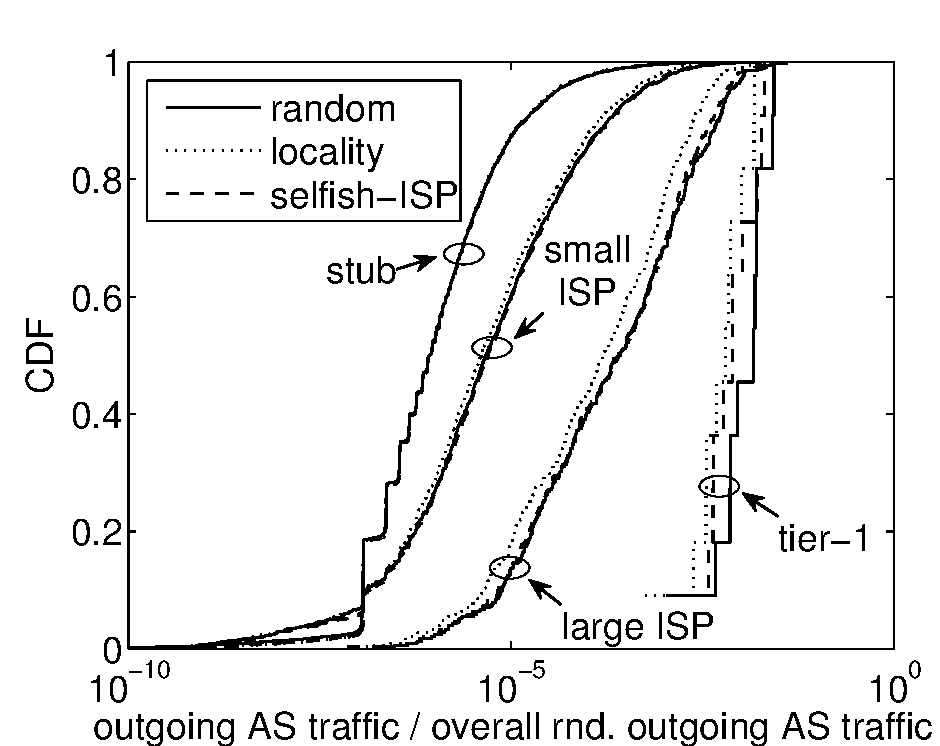
\includegraphics[width=0.7\textwidth]{aslevel/p2p/results/figs/outgoing_CDF}
 	\caption{CDF of the outgoing AS traffic grouped by AS size.}
 	\label{fig:outgoing_CDF}
\end{figure}

% \begin{figure}[bt]
% 	\centering
% 	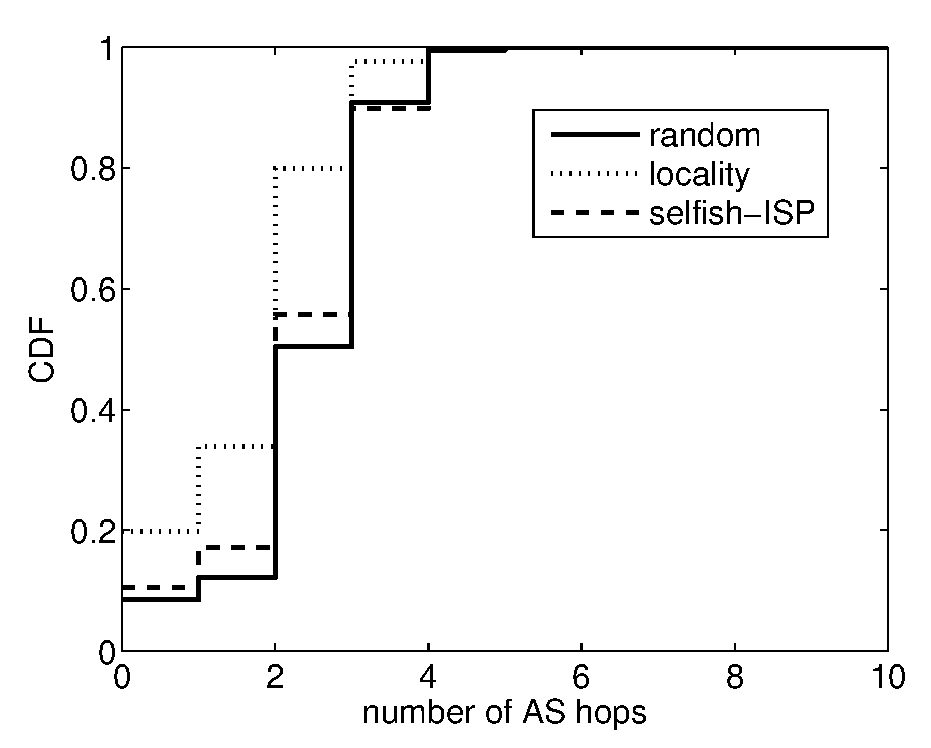
\includegraphics[width=\figwidth\textwidth]{figs/CDF_hops.eps}
%  	\caption{Cumulative probability of the number of AS hops for different peer selection strategies.}
%  	\label{fig:CDF_hops}
% \end{figure}

% \begin{figure}[bt]
% 	\centering
% 	\includegraphics[width=\figwidth\textwidth]{figs/outgoing.eps}
%  	\caption{Total outgoing AS traffic for different peer selection strategies. The outgoing traffic is normalized by the overall outgoing traffic for random peer selection.}
%  	\label{fig:outgoing}
% \end{figure}

% \begin{figure}[bt]
% 	\centering
% 	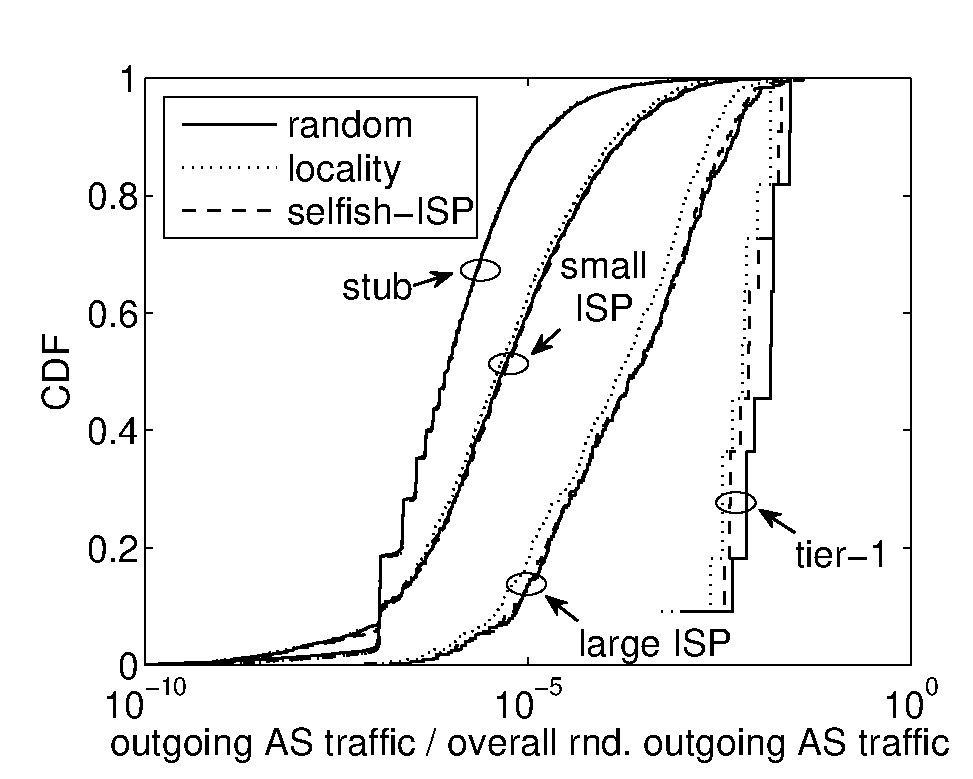
\includegraphics[width=\figwidth\textwidth]{figs/outgoing_CDF.eps}
%  	\caption{Cumulative probability of the outgoing AS traffic. The outgoing traffic is normalized by the overall outgoing traffic for random peer selection.}
%  	\label{fig:outgoing_CDF}
% \end{figure}

If we use the local selection strategy, the probability for shorter AS paths is higher, compared to random and selfish selection. If local peer selection is used, about \unit[20]{\%} of the traffic can be exchanged in the same AS, i.e. with no AS hop, which is twice as much as for the other strategies. Random and selfish selection have a median of two AS hops, whereas paths have two or less AS hops in about \unit[80]{\%} with local selection strategy. Selfish selection has no considerable potential to reduce the AS path length.

\reffig{fig:outgoing} shows the amount of inter-AS traffic produced by BitTorrent swarms. We estimate the outgoing traffic of each AS with $out(\alpha)$ in \refequ{equ:outgoing}, i.e. the load produced by all peer-to-peer connections on the links connecting $\alpha$ normalized by the number of neighbors and the number of paths sharing the links. The outgoing traffic of each BitTorrent swarm and each AS is calculated and summed up for the different AS types. For each AS type \reffig{fig:outgoing} depicts the sum of outgoing traffic normalized by the overall total outgoing traffic produced by random selection of all AS types. The peer selection strategy is coded in the different levels of grey. Independent of the selection strategy, most of the traffic is at large ISPs. Less than half of large ISP traffic is at small ISPs. The traffic going out of all the stub ASs is in total a similar amount as the traffic going out of the 11 \tier ASs. Hence, most traffic is going out of \tier ASs on a per AS basis.

We use the outgoing traffic as a measure for the load on the network.
Figure~\ref{fig:outgoing} depicts the outgoing traffic for the different selection strategies dependent on the AS type. Locality selection reduces the amount of emerging inter-AS traffic in every AS type. Especially large ISPs have a high potential to take load of inter-AS links by selecting local peers. Selfish peer selection reduces the traffic going out of \tier ASs, probably because less customers use them as transit providers and route their traffic to customers or keep it local. Apart from that selfish selection does not reduce the load on the network significantly.

Figure~\ref{fig:outgoing_CDF} shows the cumulative distribution function of the outgoing AS traffic grouped by the AS type. The outgoing traffic is normalized by the overall outgoing AS traffic of the random peer selection strategy. AS mention before \tier ASs have most outgoing traffic on a per AS basis. Further on we observe that the outgoing traffic decreases with size of the AS. Also noticeable is that with the locality peer selection algorithm we get less outgoing traffic, especially for large ISPs. The difference is not very big for a single AS, but the large number of ASs makes a big difference in the total outgoing AS traffic.

\subsubsection{Transit Costs}

We estimate the transit costs emerged by BitTorrent traffic for the different ISPs and show the potential to save costs and maximize revenues of the peer selection algorithms. We use the overall revenues for random selection, i.e., the sum of total revenues of all AS types, to normalize the values derived in this section. As the overall total balance is zero, the overall total revenues equal the overall total costs.
As described in \refsec{sec:p2p:methodology} every customer/provider AS $\alpha$ on an AS path connecting peers is charged by $\pm L(\alpha,\beta)$.

\begin{figure}[bt]
	\centering
	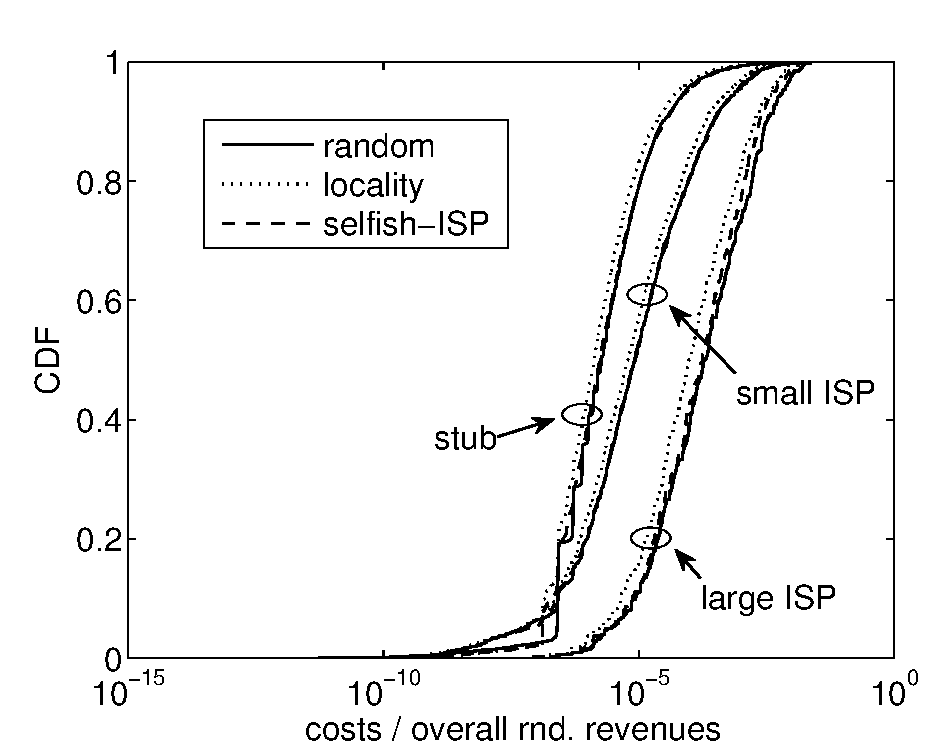
\includegraphics[width=0.7\textwidth]{aslevel/p2p/results/figs/costs_CDF}
 	\caption{Cumulative probability of normalized transit costs for different peer selection strategies. The transit costs are grouped by AS types.}
 	\label{fig:costs_CDF}
\end{figure}

\begin{figure}
	\centering
	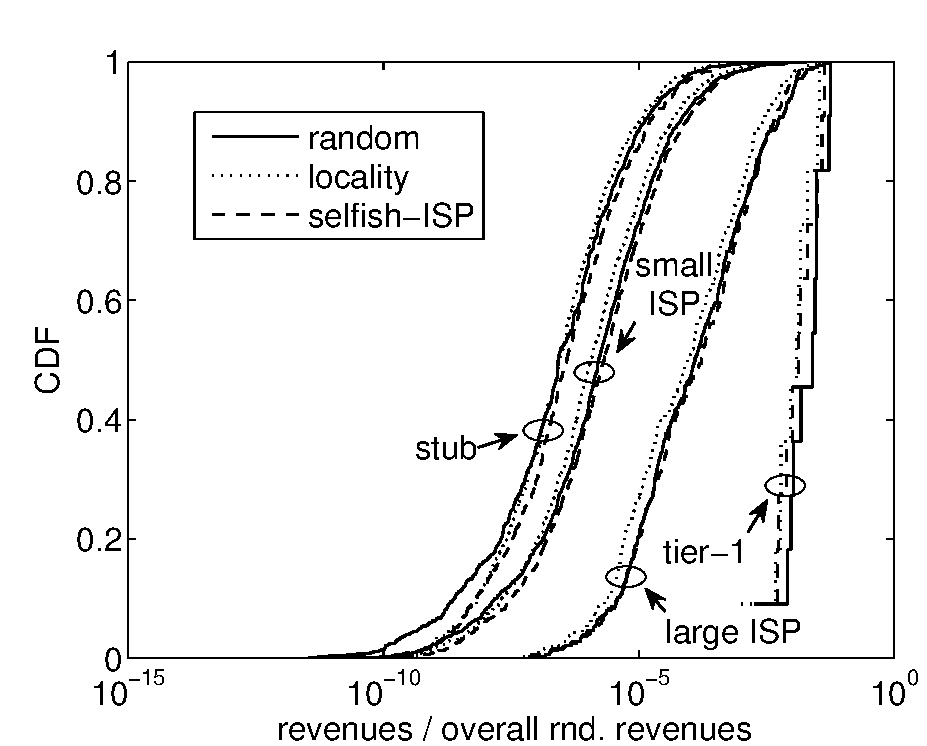
\includegraphics[width=0.7\textwidth]{aslevel/p2p/results/figs/revenues_CDF}
 	\caption{Cumulative probability of normalized revenues for different peer selection strategies. The revenues are grouped by AS types.}
 	\label{fig:revenues_CDF}
\end{figure}


Figure~\ref{fig:costs_CDF} shows the cumulative distribution function of transit costs, as calculated in \refequ{equ:costs}, for the ASs grouped by AS types. Hence, the amount ASs pay providers for transit services. The costs are normalized by the overall revenues of random selection. \tier ASs do not have providers and therefore no transit costs. Local peer selection reduces the transit costs, regarding the overall distribution of costs, for all non \tier AS types. Costs of large ASs, i.e., ASs that have many customers and forward a lot of traffic, tend be higher.

% \begin{figure}[bt]
% 	\centering
% 	\begin{subfigure}[b]{0.49\textwidth}
% 	  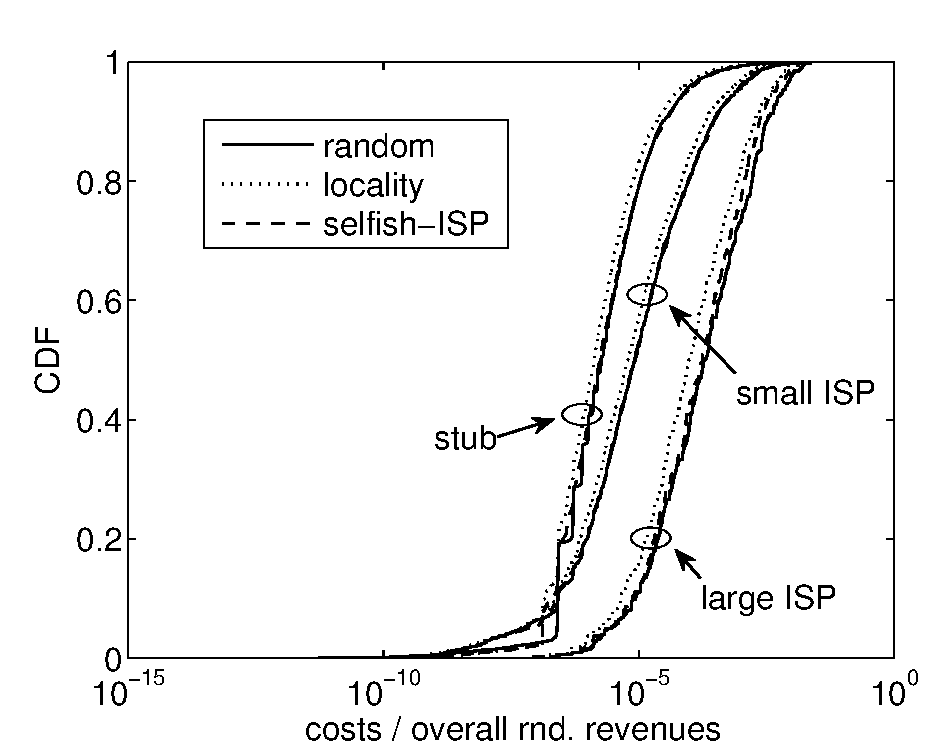
\includegraphics[width=\textwidth]{aslevel/p2p/results/figs/costs_CDF}
%     \caption{Costs}
%     \label{fig:costs_CDF}
% 	\end{subfigure}
% 	\begin{subfigure}[b]{0.49\textwidth}
% 	  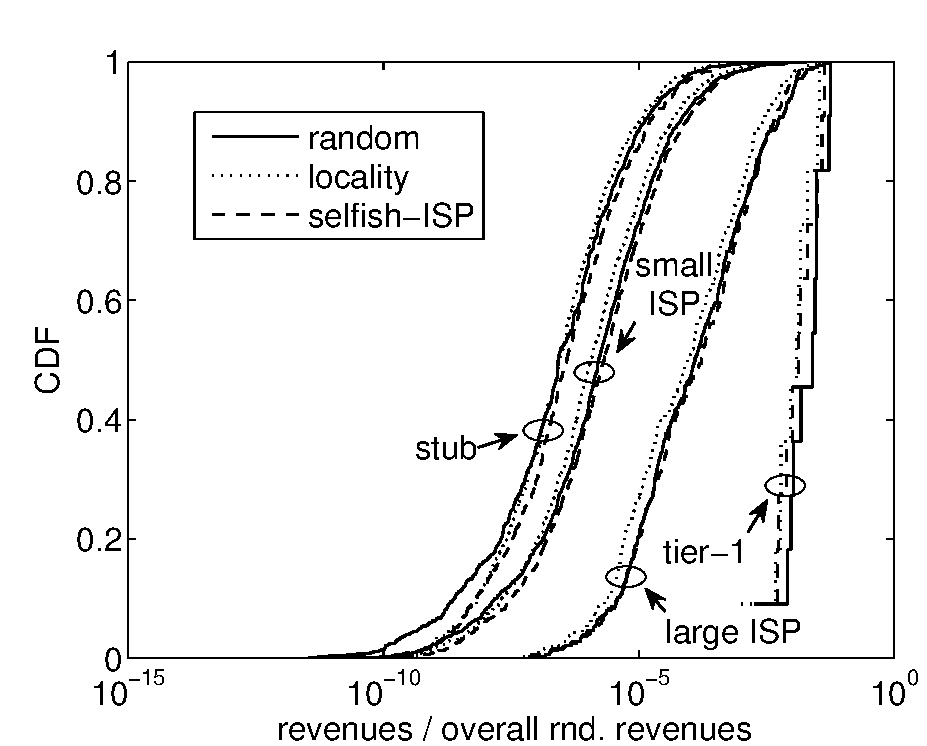
\includegraphics[width=\textwidth]{aslevel/p2p/results/figs/revenues_CDF}
%     \caption{Revenues}
%  	 	\label{fig:revenues_CDF}
% 	\end{subfigure}
%  	\caption{Cumulative probability of transit costs (left) and revenues (right) normalized by the overall revenue for random peer selection grouped by AS size.}
% \end{figure}

Figure~\ref{fig:revenues_CDF} shows the cumulative probability of revenues, see \refequ{equ:revenues}, of the ASs grouped by AS type. \Tier ASs achieve highest revenues. They have the largest customer tree which pay for transit services. ASs with a smaller customer tree get less revenues. The difference between the selection strategies is small for every single AS, but the large number of ASs makes a big difference in the total revenues and further total balance, as we explain in the next paragraph. However, we observe that stub ASs, small and large ISPs tend to have lower revenues using locality selection compared to random selection. In contrast revenues increase with higher probability for selfish-ISP selection in large intervals, in particular from $10^{-8}$ to $10^{-4}$ for stub and small ISPs. This was the aim of the selfish-ISP selection strategy. \Tier ISPs are loosing revenues if selection strategies are used. Hence, peer-to-peer guidance and selfish-ISP selection are not beneficial for \tier.

\begin{figure}[bt]
	\centering
	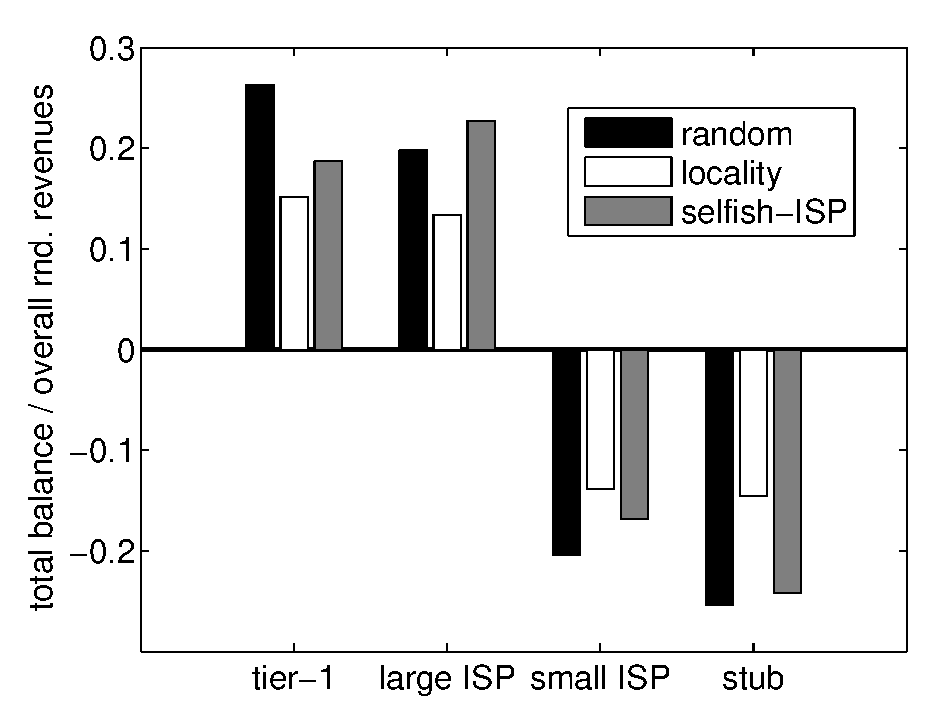
\includegraphics[width=0.7\textwidth]{aslevel/p2p/results/figs/total_balance}
 	\caption{Total balance of transit costs and revenues normalized by the overall revenue for random peer selection.}
 	\label{fig:total_balance}
\end{figure}

\begin{figure}[bt]
	\centering
	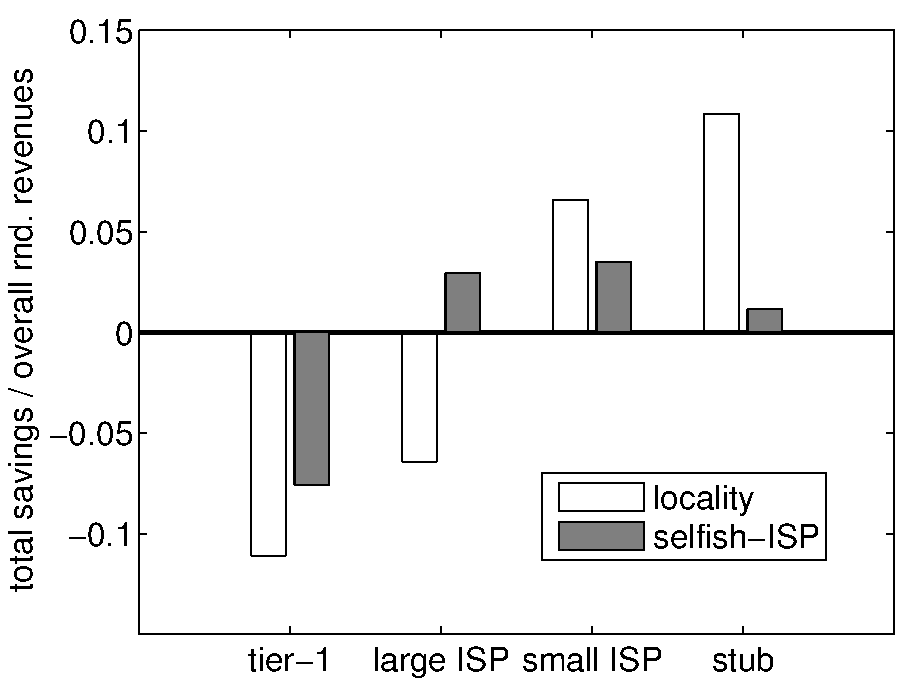
\includegraphics[width=0.7\textwidth]{aslevel/p2p/results/figs/savings}
 	\caption{Total savings of locality and selfish-ISP selection strategy over random peer selection normalized by the overall revenue for random selection.}
 	\label{fig:savings}
\end{figure}

The total balance overall measured BitTorrent swarms is calculated by subtracting costs from revenues of each AS. Figure~\ref{fig:total_balance} depicts the total balance depending on the AS size. The total balance is normalized by the overall revenues of random selection. The balance is calculated for the standard BitTorrent peer selection, the locality-aware and selfish strategy.
For all three strategies, \tier and large ISPs have a positive balance and small ISP and stub ASs have a negative balance. This corresponds to the expectation, since \tier and large ISPs have many customers whereas small ISPs and stub ASs have many providers. Hence, small ASs have to pay for the transit provided by large ASs.

To highlight the effect of the peer selection strategies on the balance of the ASs, we investigate the savings over random selection.
Comparing the local strategy with the standard strategy, we notice that small ASs save costs by selecting local neighbors, resulting in less revenues by the large ASs.
Figure~\ref{fig:savings} shows the savings over random selection achieved by using locality and selfish-ISP selection. The savings are calculated by subtracting the total balance with selection strategy from the total balance of the random selection strategy. The savings are normalized by the overall revenues of random selection. \tier ASs loose most revenue when local selection is used, which is \unit[10]{\%} of the overall total revenue. The traffic is kept locally and less traffic is forwarded by \tier ASs to reach remote destinations. Hence, the transit services of \tier ASs are avoided which results in less revenues. Large ISPs also gain less when local peer selection is used. Small ISPs and stub ASs gain from local peer selection, since they save costs for transit services by avoiding long AS paths. \unit[10]{\%} of the overall total costs are saved by stub ASs, hence they have the highest potential to profit from selecting peers by locality.

% \begin{figure}[bt]
% 	\centering
% 	\begin{subfigure}[b]{0.49\textwidth}
% 	  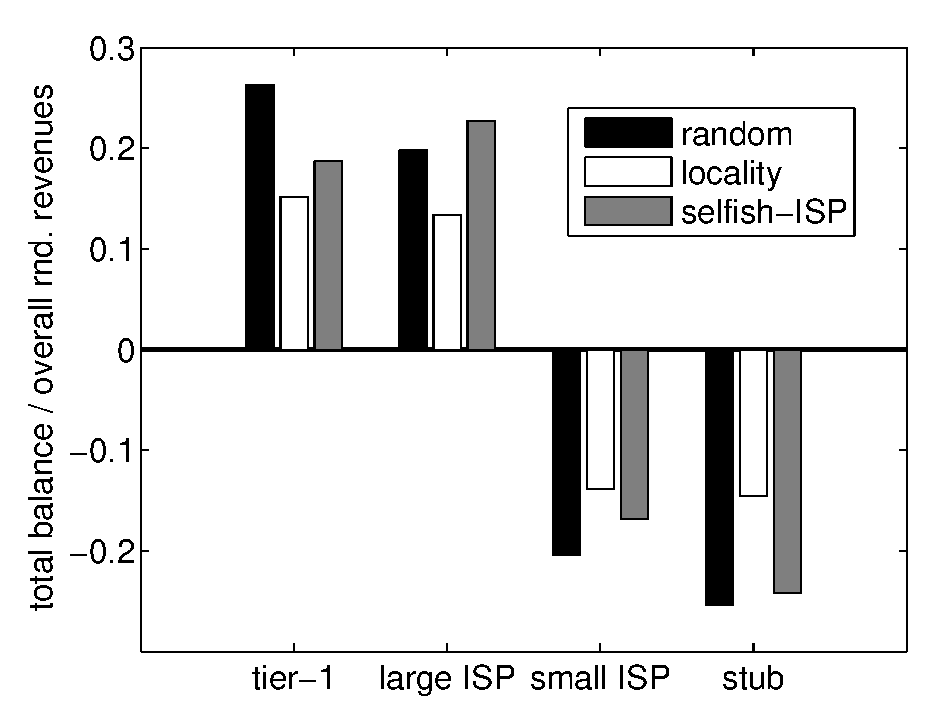
\includegraphics[width=\textwidth]{aslevel/p2p/results/figs/total_balance}
%     \caption{Balance}
%     \label{fig:total_balance}
%   \end{subfigure}
% 	\begin{subfigure}[b]{0.49\textwidth}
% 	 	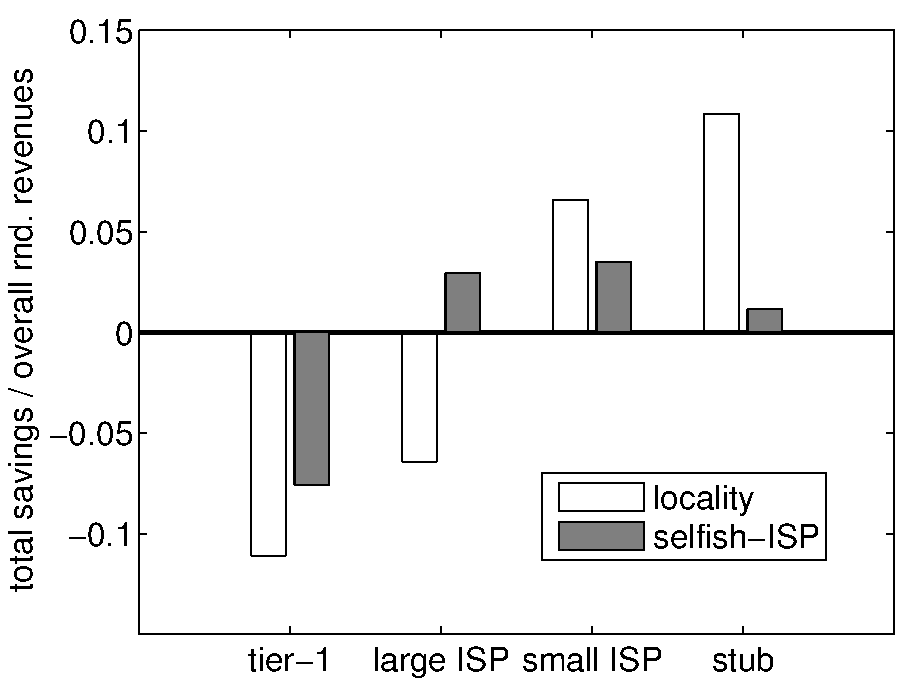
\includegraphics[width=\textwidth]{aslevel/p2p/results/figs/savings}
%     \caption{Savings}
%     \label{fig:savings}
% 	\end{subfigure}
% 	\caption{Total balance of transit costs (left) and total savings over random selection (right) normalized by the overall revenue for random peer selection.}
% \end{figure}


The only way to increase the prospect on higher profit for large ISPs is using the selfish strategy. But also small ISPs have a high potential to maximize their revenues being selfish. Thus, large and small ISPs are in a win-win situation, since they can connect to their plenty customers and do not have to pay for transit services by avoiding connections to providers. This is where \tier ASs loose, since less of the ISPs use them as provider in the selfish strategy. Thus, a \tier AS cannot be more selfish than in the random selection strategy. Having only few or no customers, stub ASs have poor capabilities to be selfish but avoiding providers also gives them a small advantage over random selection.

%The main winners using the selfish selection strategy are large ISPs. As explained before, the customer tree of large ISPs is large, thus large ISPs can maximize there win, while avoiding customer to provider links to \tier ASs. This is probably also the reason that if selfish selection is used, Tier1 ASs loose most compared to random peer selection.

%    1.0e+04 *
%    -1.6933   -0.0151    0.0058    0.0027
%    -1.0110    0.0597   -0.0010   -0.0006
%For Stub ASs peer selection is not interesting, since they do not have a choice and have to connect to their providers to reach other peers, except of those of the same AS. Hence, Stub ASs save a little if they use the local strategy. For Tier1 ASs the investigated mechanisms are of disadvantage. First, Tier1 ASs barely have peers and therefore cannot influence the peer selection behavior in the swarms. Second, Tier1 ASs usually gain of transit traffic, but transit traffic is avoided by the peer selection mechanisms. Small and large ISPs have the greatest cost saving potential. ASs with many customers, i.e. large ISPs, profit of the selfish selection strategy by prioritizing connections to customer ASs. Small ISPs can save costs by keeping the traffic local and avoiding customer to provider links.
